\documentclass[11pt]{article}
\title{assignment01}
\author{Seung Yeop, Seon (20144753)}
\usepackage[a4paper, top=2.5cm, bottom=2.5cm, left=2.2cm, right=2.2cm]%
{geometry}
\usepackage{graphicx}%
\usepackage{hyperref}

%% Language and font encodings
\usepackage[english]{babel}

%% Sets page size and margins
\usepackage[a4paper, top=2.5cm, bottom=2.5cm, left=2.2cm, right=2.2cm]%
{geometry}

\begin{document}
\maketitle
\section{Introduction}
 This Document is dealing with how to use Git and benefits from utilizing it.
\section{The explantions of Git's commands}
	\subsection{Put your personal informations}
	-Before doing any operation, put your email and name. When you collaborate with others, This informations are very useful for checking who wrote the code.

	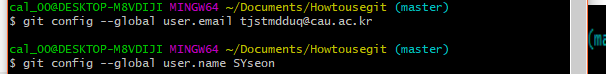
\includegraphics[height=3cm, width=14cm]{c02.PNG}

	\subsection{Importing a new project}
	-At first, enter the above code \textbf{cd address}. then, you can get in the folder named \textbf{Howtousegit}. Second, \textbf{git init} makes local repository in your folder. Third,  \textbf{git add} makes your files in the folder are going to store in a temporary staging area which Git calls the "index".

	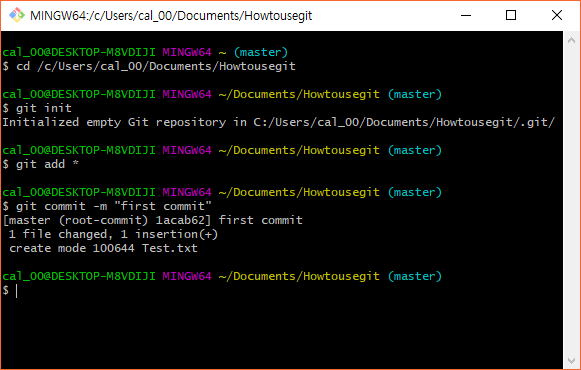
\includegraphics[height=7cm, width=14cm]{c01.PNG}

	\pagebreak	
	\subsection{Committing your files}
	You can permanently store the contents of the index in the repository by using git commit. Let's take a look at some useful code related to git commit.

	-Through the following code, we can see if the file has been modified. If you use this code before you commit, it will be useful.

	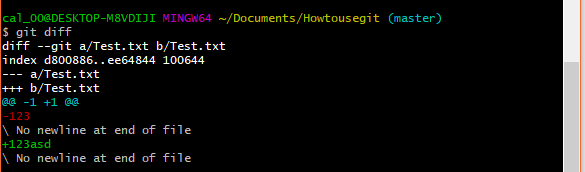
\includegraphics[height=5.3cm, width=14cm]{gitdiff.PNG}
	
	-Using \textbf{git status}, you can check the status about the commit.

	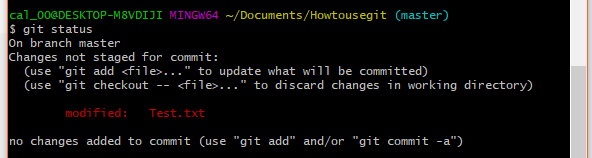
\includegraphics[height=5.3cm, width=14cm]{gitstatus.PNG}

	-Now, we are committing. \textbf{-m} means to leave messages. If you don't this method, error will be raised.

	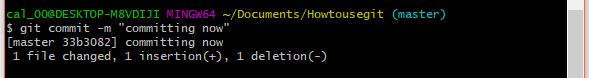
\includegraphics[height=2.5cm, width=14cm]{gitcommit.PNG}

	-Or you can use this method. If you use this method, you don't need to add your files before committing.

	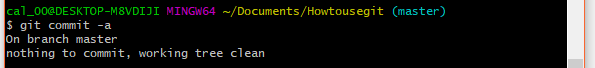
\includegraphics[height=2.5cm, width=14cm]{gitcommita.PNG}

	\pagebreak
	\subsection{Viewing project history}
	You can see the history of changing.
	
	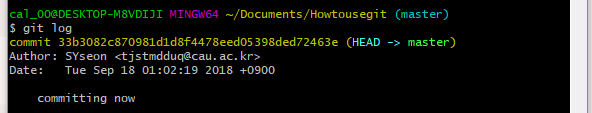
\includegraphics[height=2.5cm, width=14cm]{gitlog.PNG}
	
	-Also, by using \textbf{git log -p}, you can see whole changes of your files.

	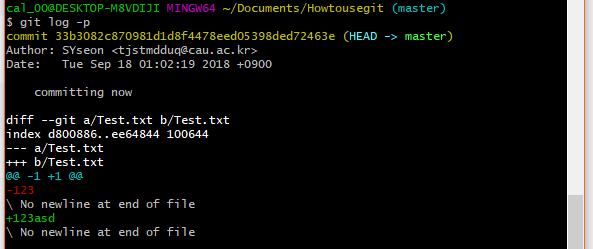
\includegraphics[height=2.5cm, width=14cm]{gitlogp.PNG}
	
	\subsection{Branch}
	If you use branch, you can move to the point you specified. Let's look at how to use branch.

	-Before committed, I created \textit{Test.txt} and this file contained the following messages.

	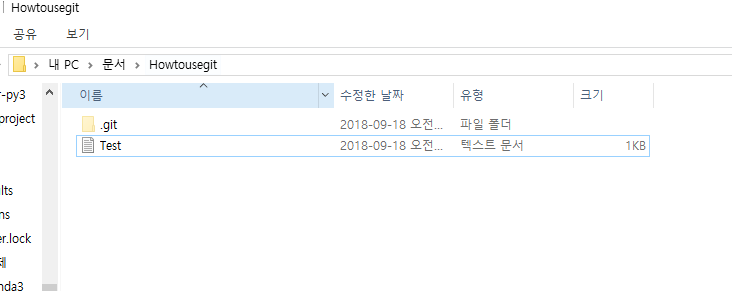
\includegraphics[height=5.5cm, width=14cm]{branch.PNG}
	
	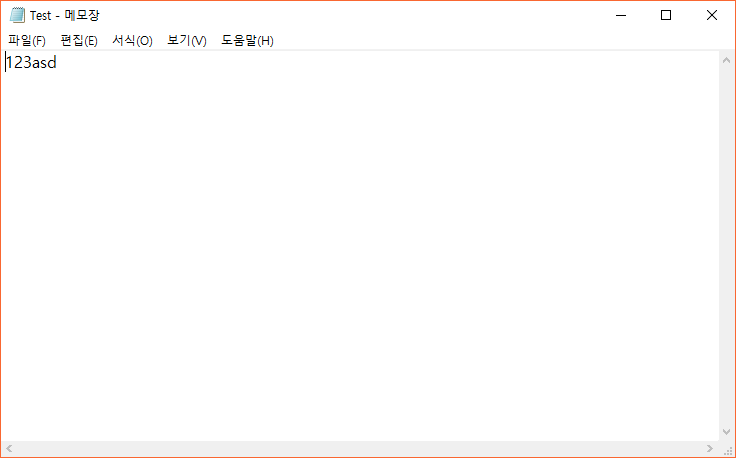
\includegraphics[height=7cm, width=10cm]{branch00.PNG}
	\pagebreak
	
	-Now, I am changing contents of the file.	

	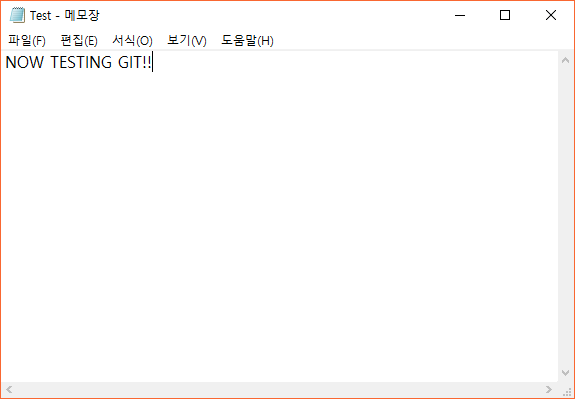
\includegraphics[height=7cm, width=10cm]{branch01.PNG}
	
	-And entering the following commands.

	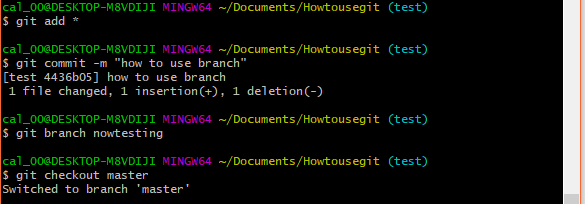
\includegraphics[height=7cm, width=10cm]{branch02.PNG}
	
	-We can see the file returns to first state. The master branch is the point at which the contents of the text file are saved before making changes. The nowtesting branch, on the other hand, is when the contents of the text file are saved after the change. We can move to the desired point through the branch.

	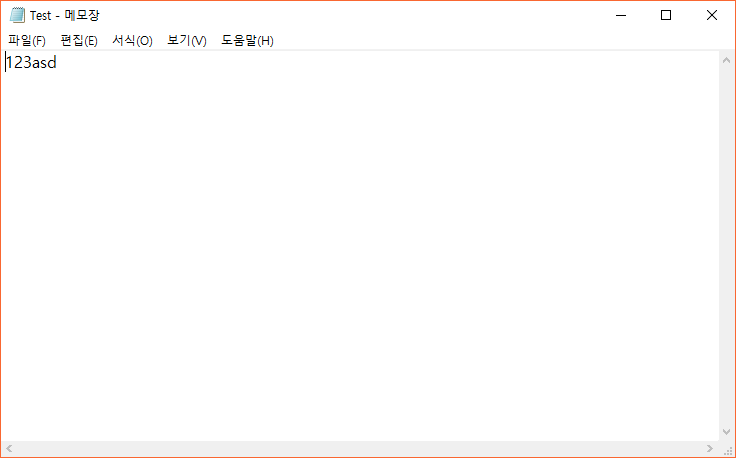
\includegraphics[height=7cm, width=10cm]{branch00.PNG}
	
	\subsection{To access GitHub}
		\subsubsection{git pull}
		 \textbf{Git pull} merges the changes from Machine-learning-for-bio-data’s "master" branch into Pull’s current branch.	
		
		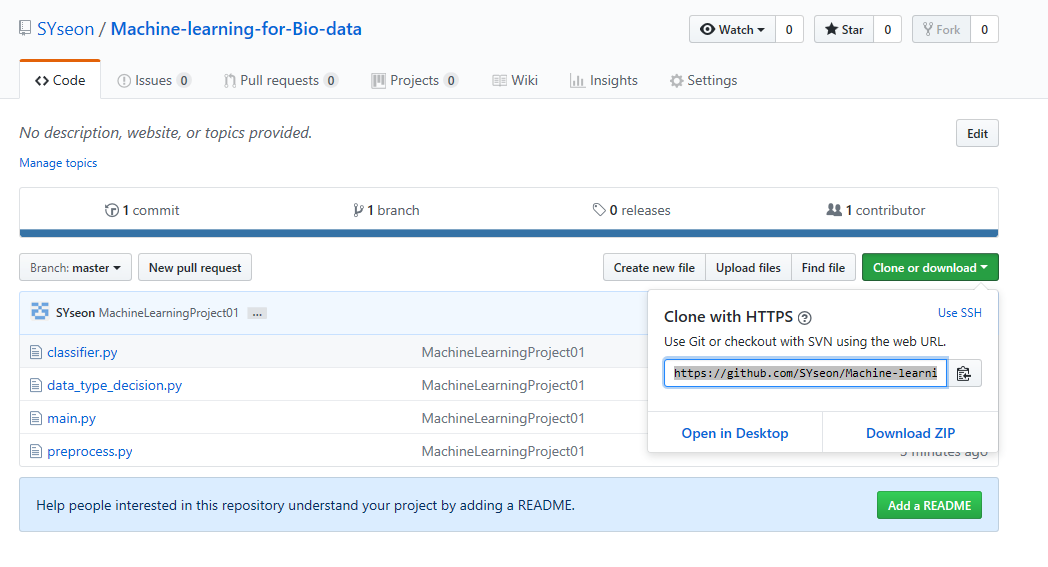
\includegraphics[height=7cm, width=14cm]{gitpull01.PNG}
		
		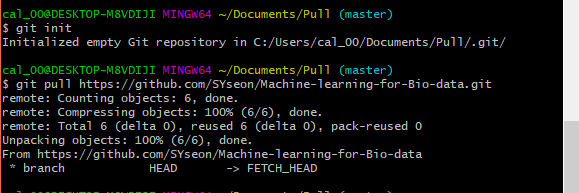
\includegraphics[height=7cm, width=14cm]{gitpull02.PNG}
		
		
\includegraphics[height=7cm, width=14cm]{gitpull03.PNG}

		\subsubsection{git clone}
		\textbf{Git clone} creates a new directory "Machine-learning-for-bio-data containing a clone of The Clone’s repository. The clone is on an equal footing with the original project, possessing its own copy of the original project’s history.
		
		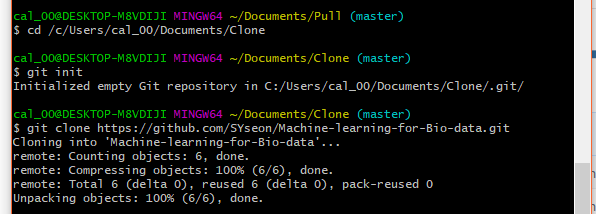
\includegraphics[height=7cm, width=14cm]{gitclone01.PNG}
		
		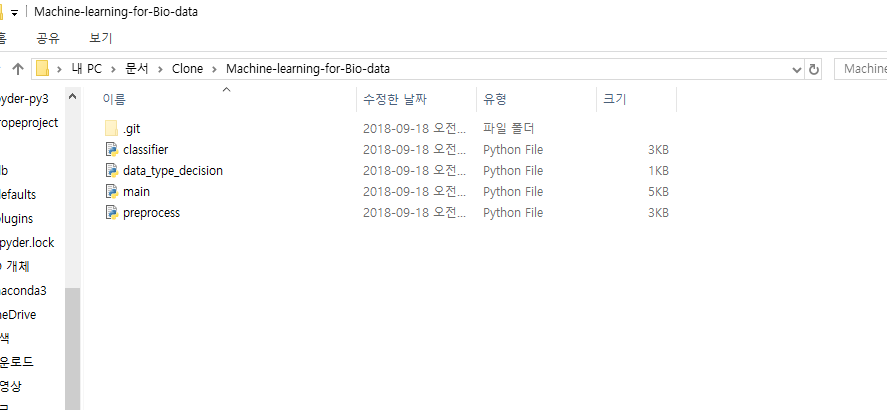
\includegraphics[height=7cm, width=14cm]{gitclone02.PNG}
		\pagebreak
		
		\subsubsection{git remote}
		It defines repository's name.
		
		
\includegraphics[height=1.7cm, width=14cm]{gitremote.PNG}
		
		\subsubsection{git fetch}
		\textbf{Git fetch} brings the source of the remote repository to the local repository. However it doesn't conduct to merge. 
		
		
		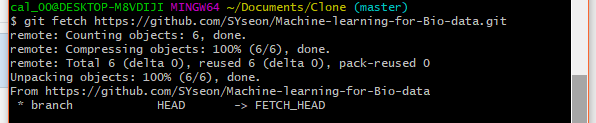
\includegraphics[height=5cm, width=14cm]{gitfetch.PNG}
		
		
		\subsubsection{git push}
		\textbf{Git push} updates remote repository using local repository, while sending objects necessary to complete the given repository.
		
		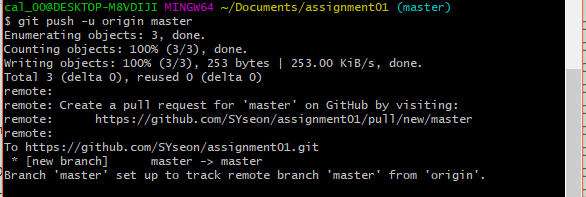
\includegraphics[height=7cm, width=14cm]{gitpush.PNG}

\pagebreak
\section{The benefits from using Git}
Now, Let's talk about the advantages of Git using the features mentioned above.
	\subsection{Collaborating}
	In the above section, we can see that commit our branch in the local repository to the remote repository. Also, saw the reverse case. Through these processes, we can share our code with our colleagues instantly.
	\subsection{Version control}
	When you are programming, there are situations to code in a completely different way than the previous one. and sometimes you make mistakes. If you do not use git, this is pretty bothering. However, with git, you just have to go back to the previous branch.
	\subsection{The most popular code management tools}
	It's a big advantage that GitHub is the most popular code management tool. The vast majority of developers work with GitHub, we can only use GitHub to collaborate with other developers. Also, due to this trait, GitHub has a huge amount of open source. We can free access to open source.

\section{GitHub link}
\href{https://github.com/SYseon/assignment01}{https://github.com/SYseon/assignment01}

\end{document}